
\documentclass[11pt]{article}

\usepackage{amsmath}
\usepackage{amssymb}
\usepackage[top =1 in  , bottom =1 in , left=0.5 in , right = 0.5 in]{geometry}
\usepackage{graphicx}
\newcommand{\BibTeX}{{\sc Bib}\TeX}
\usepackage{url}
\begin{document}
\nocite{*}


\title {CS296 Project: Torpedo Boat Destroyer System}
\author {\emph{Group 13} \\
	\emph{Pintu Lal Meena} \\
	 \textrm{120050018} ,  \textsf{pintulalmeena@hotmail.com} \\
	\emph{Pranay Dhondi } \\
	\textrm{120050054} , \textsf{pranaydhondi@gmail.com} \\
	\emph{Shivam Garg}\\
	\textrm{12D020036} , \textsf{shivam.garg55@gmail.com}}
\date{\today} 
\maketitle
\section{Introduction}
This report discusses the simulation of torpedo boat destroyer system made using box2d.  We have used keyboard to control the simulation. 
\section{Design Analysis}
The most interesting thing about our design is we have simulated such a complex looking 
machines easily using prismatic joints, revolute joints and impulses in Box2d.
\subsection{Parts of the Simulation}
\subsubsection{Moving Boxes}
 \begin{center}
 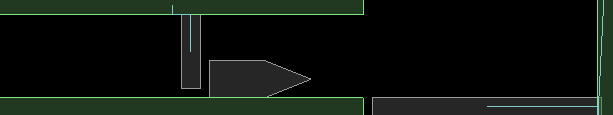
\includegraphics[scale=0.5]{images/push}
 \end{center}
We have used prismatic joints between boxes and horizontal surfaces to push parts of torpedo from surface to lift, to push torpedo from one lift to
another and to torpedo launcher.
\subsubsection{Torpedo}
\begin{center}
 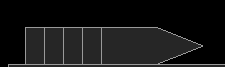
\includegraphics[scale=0.5]{images/torpedo}
 \end{center}
We have made torpedo using 4 boxes and one conical polygon.
\subsubsection{Lifts}
\begin{center}
 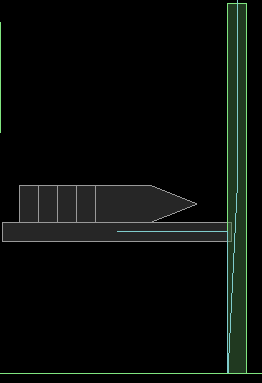
\includegraphics[scale=0.5]{images/lift}
 \end{center}
We carry the torpedo up from ground to the launcher using 2 lifts. These lifts
slide along vertical walls. We have implemented this using prismatic joints.
\subsubsection{Torpedo Launcher}
\begin{center}
 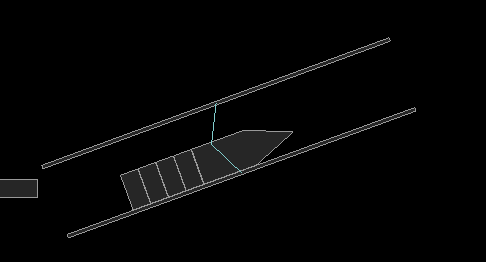
\includegraphics[scale=0.5]{images/launcher}
 \end{center}
The torpedo launcher is made using two box shapes which independently rotate about a fixed body (using revolute joint). 
We haven't made any fixture for this fixed body, so it is not visible. Although torpedo is made up od 5 different bodies, but when they reach 
the torpedo launcher they behave like a single body. This is achieved by increasing friction on the base of the launcher, so that
when launcher rotates these bodies do not  fall apart.We have used linear impulses to shoot the torpedo. Linear impulse is also used to make the hind section of the torpedo fall down during
the motion of torpedo in the air.
\subsection{Difference between original design and simulation}
There is not much of difference between the basic design of our simulation and original design.
We have implemented some of the movements in a different manner and added some new things to the simulation also
which are discussed below:
 \begin{center}
 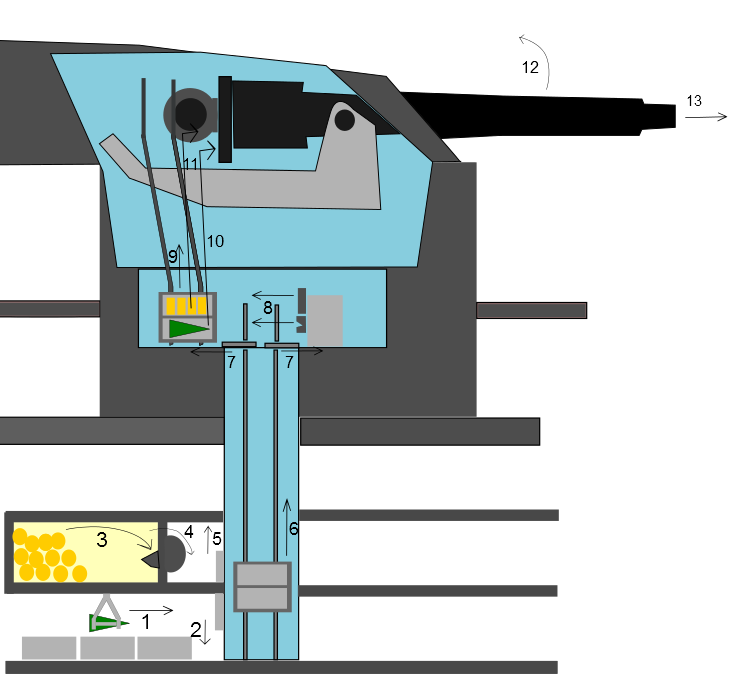
\includegraphics[scale=0.3]{images/original}
 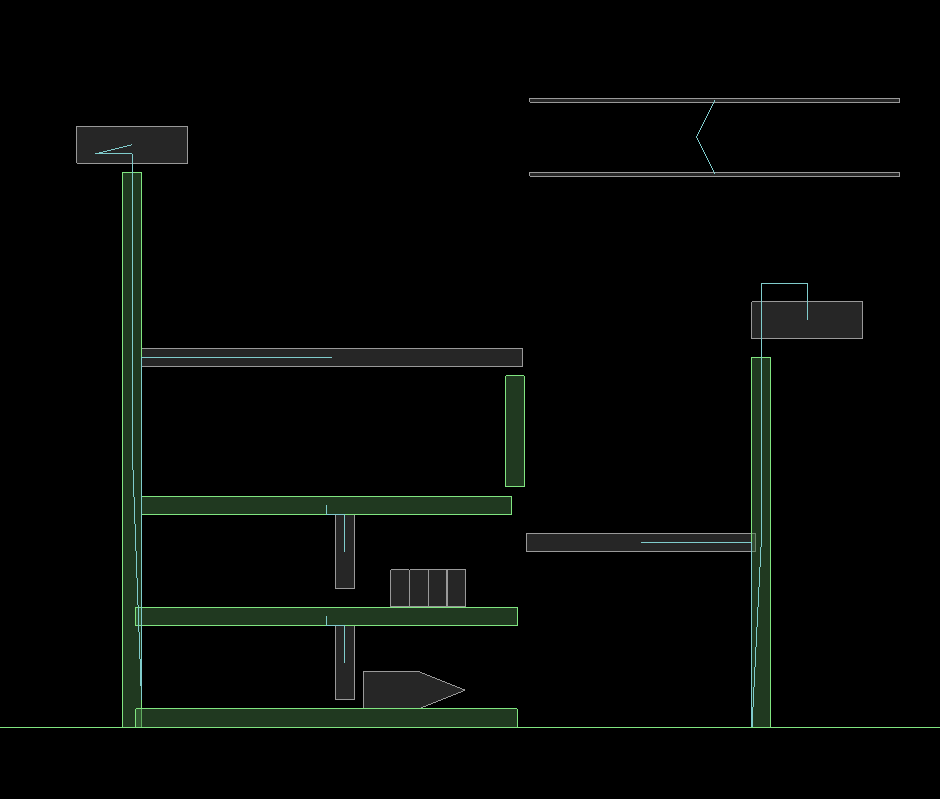
\includegraphics[scale=0.25]{images/simulation}
 \end{center}
 \hspace{100 pt}{\it Original Design} \hspace{150 pt}{\it Design made in Box2d} \\\\
In the original design, cone and the hind section of the torpedo is transferred to lift in a slightly different manner than we implemented it.
It is because, many parts of the original simulation transfer mechanism were not practically implementable in Box2d. We have kept the hind section and
the conical part on the same level on lift whereas in the original design, they were present on two different levels.
In our simulation we have also shown the motion of torpedo after being shot (this is not a part of original simulation).
\section{Timing Experiment Analysis}
This section includes the observations and inferences from timing experiments and graphical analysis of these experiments.

\subsection{Observations}
\begin{itemize}
\item Loop Time first increases, then decreases and then finally increases as we increase the number of iterations
\begin{center}
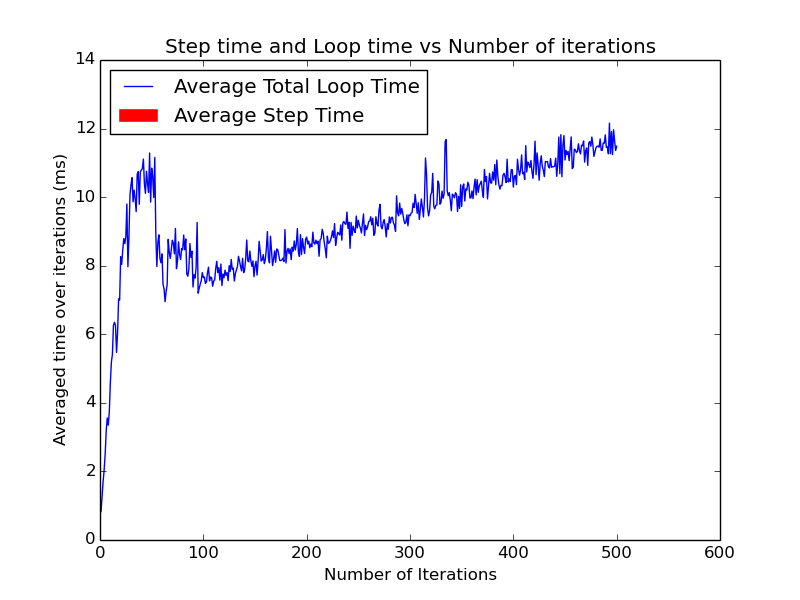
\includegraphics[scale=0.45]{images/g13_plot01}
\end{center}
\item Average Step time decreases exponentially as we increase the number of iterations 
\item Velocity update Time $>$ Collision time $>$ Position Update Time
\item Step Time is greater than sum of collision, position update and velocity update time
\begin{center}
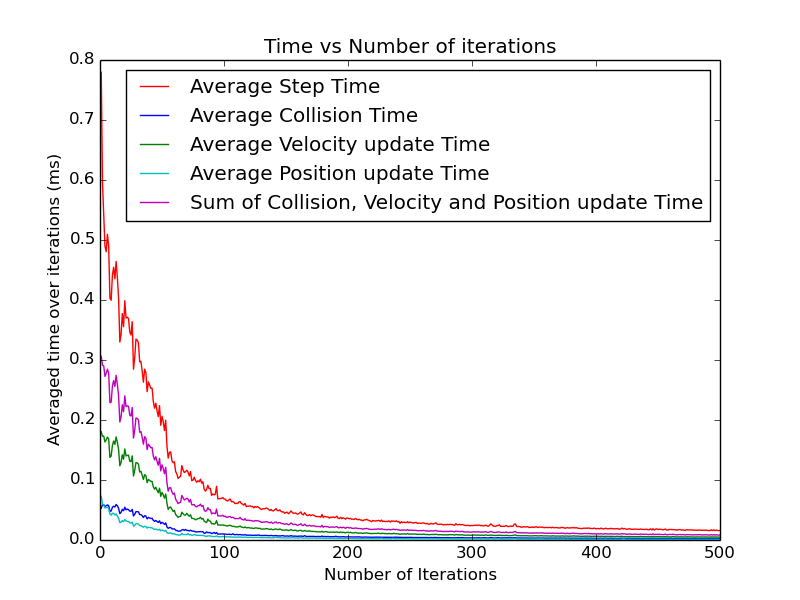
\includegraphics[scale=0.45]{images/g13_plot02}
\end{center}
\item Variation in average step time decreases as we increase the number of iterations
\begin{center}
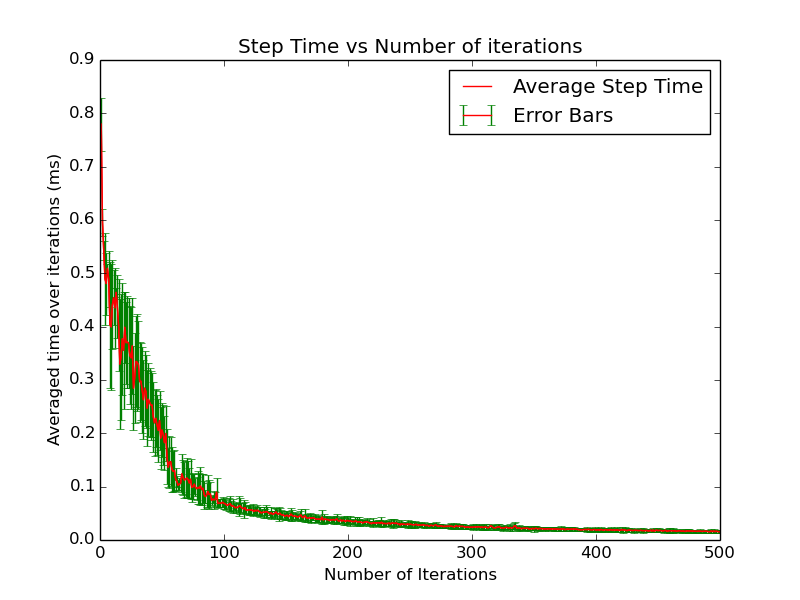
\includegraphics[scale=0.45]{images/g13_plot03}
\end{center}
\item Average step time over all reruns and over random reruns is almost the same for higher iteration values
\begin{center}
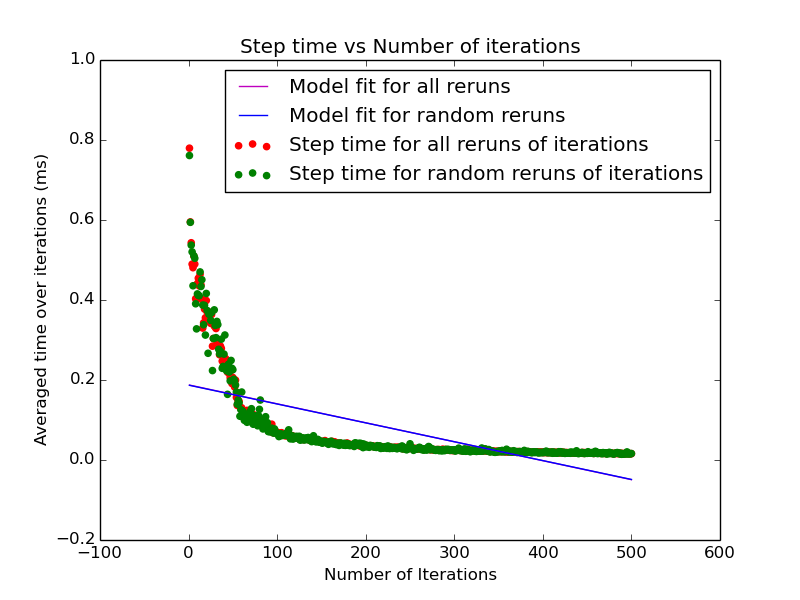
\includegraphics[scale=0.45]{images/g13_plot05}
\end{center}
\end{itemize}
 
\subsection{Reasoning and Inferences}
\begin{itemize}
\item The initial steps take more time as compared to the later steps giving rise to decrease in average step time with increase in number of iterations
\item Velocity update takes more time than collision and position update
\item Collision and position update take almost same time
\item Variation in average step time decreases because number of data points (iteration number) is increasing
\item Average step time over all reruns and randum reruns is almost same for higher iteration values because with high iteration value, variation in step time decreases, so both quantities lie near each other
\end{itemize}


\section{Code Profiling}
\begin{center}
 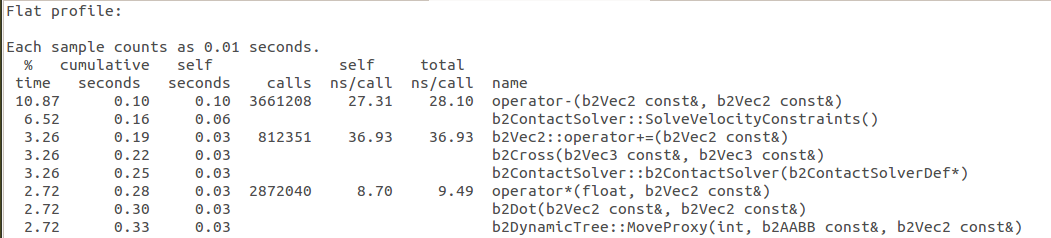
\includegraphics[scale=0.5]{images/prof1}
 \it Some part of Flat Profile
 \end{center}
  \begin{center}
 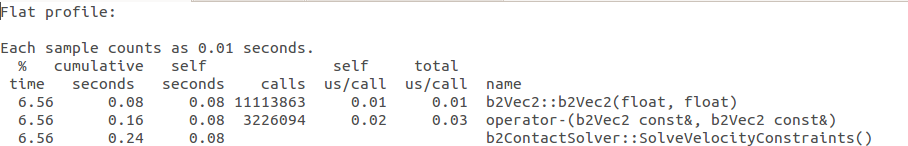
\includegraphics[scale=0.5]{images/debprof1}
 \it \\ Some part of Flat Profile in debug mode
 \end{center}
 Profiling data shows that the functions which took most of the time are \textsf{operator-(b2Vec2 const\&, b2Vec2 const\&)}, \textsf{b2ContactSolver::SolveVelocityConstraints()}
 , \textsf{b2Vec2::operator+=(b2Vec2 const\&)} and \textsf{b2Vec2::b2Vec2(float, float)}. This is possibly due to a large number of prismatic joints in our simulation. All these prismatic joints have a lower and upper 
 translation limits. As it has to be checked again and again that whether the body is in its translation limits or not, therefore number of calls to \textsf{operator-(b2Vec2 const\&, b2Vec2 const\&)} 
 is quite high. Function \textsf{b2Vec2::operator+=(b2Vec2 const\&)} is possibly called to change the coordinates of any body. \textsf{b2ContactSolver::SolveVelocityConstraints()} is called
 to solve the velocity constraints. The percentage of total time taken by this function is  usually high in all simulations because in all simulations velocity constraints have to be
 solved at each step. \textsf{b2Vec2::b2Vec2(float, float)} is mainly called by operators +,- and *. 
  \begin{center}
 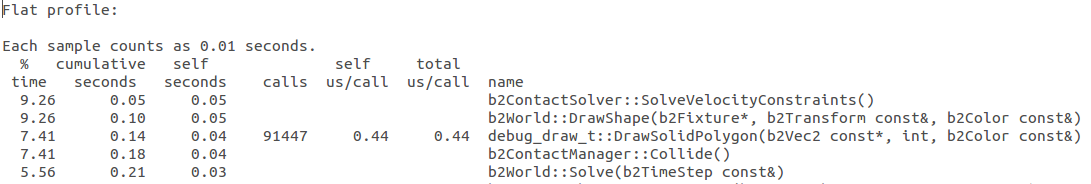
\includegraphics[scale=0.5]{images/relprof1}
 \it Some part of Flat Profile in release mode
 \end{center}
 

 In release mode, functions \textsf{DrawShape} and \textsf{DrawSolidPolygon} take most of the time apart from the function \textsf{b2ContactSolver::SolveVelocityConstraints()}. 
 These functions
 are called whenever we draw shapes(polygons). \textsf{DrawSolidPolygon} is called by the \textsf{DrawShape}.\\
 \begin{center}
 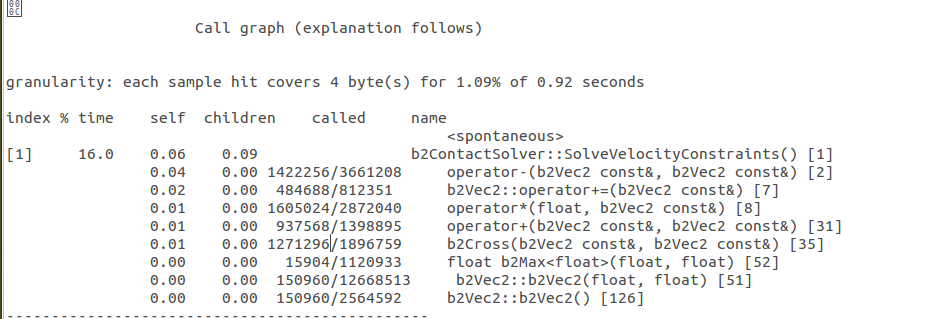
\includegraphics[scale=0.5]{images/prof2}
 \it \\Some part of Call Graph
 \end{center}
 It can be seen from this part of call graph that most of the calls to \textsf{operator-(b2Vec2 const\&, b2Vec2 const\&)} are made by \textsf{b2ContactSolver::SolveVelocityConstraints()}.
  Major portion of the time spent on this function is due to this call only. The other major caller of \textsf{operator-(b2Vec2 const\&, b2Vec2 const\&)} 
  is the function \textsf{b2FindMaxSeparation(int*, b2PolygonShape const*, b2Transform const\&, b2PolygonShape const*, b2Transform const\&)}. \textsf{b2FindMaxSeparation(int*, b2PolygonShape const*, b2Transform const\&, b2PolygonShape const*, b2Transform const\&)}
   must be called to find the separation between bodies to check if they are in translation limits or not (prismatic joint).
   We could not find any evident way to change our code so as to decrease calls to above mentioned functions as our simulation is highly dependent on prismatic joints which call
   these functions repeatedly. 
 
\bibliographystyle{plain}
\bibliography{report} 
\end{document}
